\documentclass{article}
\usepackage[left=0.5in,top=0.5in,right=0.5in,bottom=0.5in]{geometry}
\usepackage[english]{babel}
\usepackage[utf8]{inputenc}
\usepackage[table]{xcolor}
\usepackage{amssymb,amsmath,amsthm}
\usepackage{changepage,threeparttable}
\usepackage{booktabs,multirow}
\usepackage{subcaption}
\usepackage{graphicx}
\usepackage{soul}
\graphicspath{{./images/}}
\def\F#1{\(#1\)}
\title{Lab 12: The Impedance of an Inductor}
\author{Philip Kim}
\date{\today}
\begin{document}
\maketitle
\vspace*{-1cm}
\begin{table}[!htp]\centering
  \begin{tabular}{|c|c|c|c|c|c|c|}\hline
    \multicolumn{7}{|c|}{\textbf{Table 1: First Approximation for \F{R_{int}}}}\\\hline
    \F{f (Hz)}&s/DIV&\F{V_{RL} (V)}&V/DIV for \F{V_{RL}}&\F{V_{L} (V)}&V/DIV for \F{V_{L}}&\F{R_{int} (\Omega)}\\\hline
    1000&0.5ms&3.56V&0.5V&0.05V&0.5V&1.42\\\hline
  \end{tabular}
\end{table}
\begin{table}[!htp]\centering
  \begin{tabular}{|c|c|c|c|c|c|c|c|c|c|}\hline
    \multicolumn{10}{|c|}{\textbf{Table 2: First Approximation for \F{L}}}\\\hline
    \F{f (Hz)}&s/DIV&\F{V_{RL} (V)}&V/DIV for \F{V_{RL}}&\F{V_{L} (V)}&V/DIV for \F{V_{L}}&\F{I_R (A)}&\F{Z_{L,eff} (\Omega)}&\F{X_L (\Omega)}&L (H)\\\hline
    65000&0.2ms&3.28V&0.5V&0.10V&0.5V&0.033&3.05&0.771&1.89e-6\\\hline
  \end{tabular}
\end{table}
\begin{table}[!htp]\centering
  \begin{tabular}{|c|c|c|c|c|c|}\hline
    \multicolumn{6}{|c|}{\textbf{Table 3: The Impedance of an Inductor}}\\\hline
    \F{f (Hz)}&s/DIV&\F{V_{RL} (V)}&V/DIV for \F{V_{RL}}&\F{V_{L} (V)}&V/DIV for \F{V_{L}}\\\hline
    1000&0.5ms&3.56V&0.5V&0.05V&0.5V\\\hline
    22000&0.5ms&3.56V&0.5V&0.06V&0.5V\\\hline
    32000&0.5ms&3.46V&0.5V&0.08V&0.5V\\\hline
    39000&0.5ms&3.42V&0.5V&0.08V&0.5V\\\hline
    45000&0.5ms&3.38V&0.5V&0.08V&0.5V\\\hline
    50000&0.2ms&3.36V&0.5V&0.09V&0.5V\\\hline
    55000&0.2ms&3.32V&0.5V&0.09V&0.5V\\\hline
    60000&0.2ms&3.30V&0.5V&0.10V&0.5V\\\hline
    65000&0.2ms&3.28V&0.5V&0.10V&0.5V\\\hline
  \end{tabular}
\end{table}

\begin{center}
  \subsection*{SETUP}
  \begin{figure}[!htp]
    \begin{subfigure}{0.5\textwidth}
    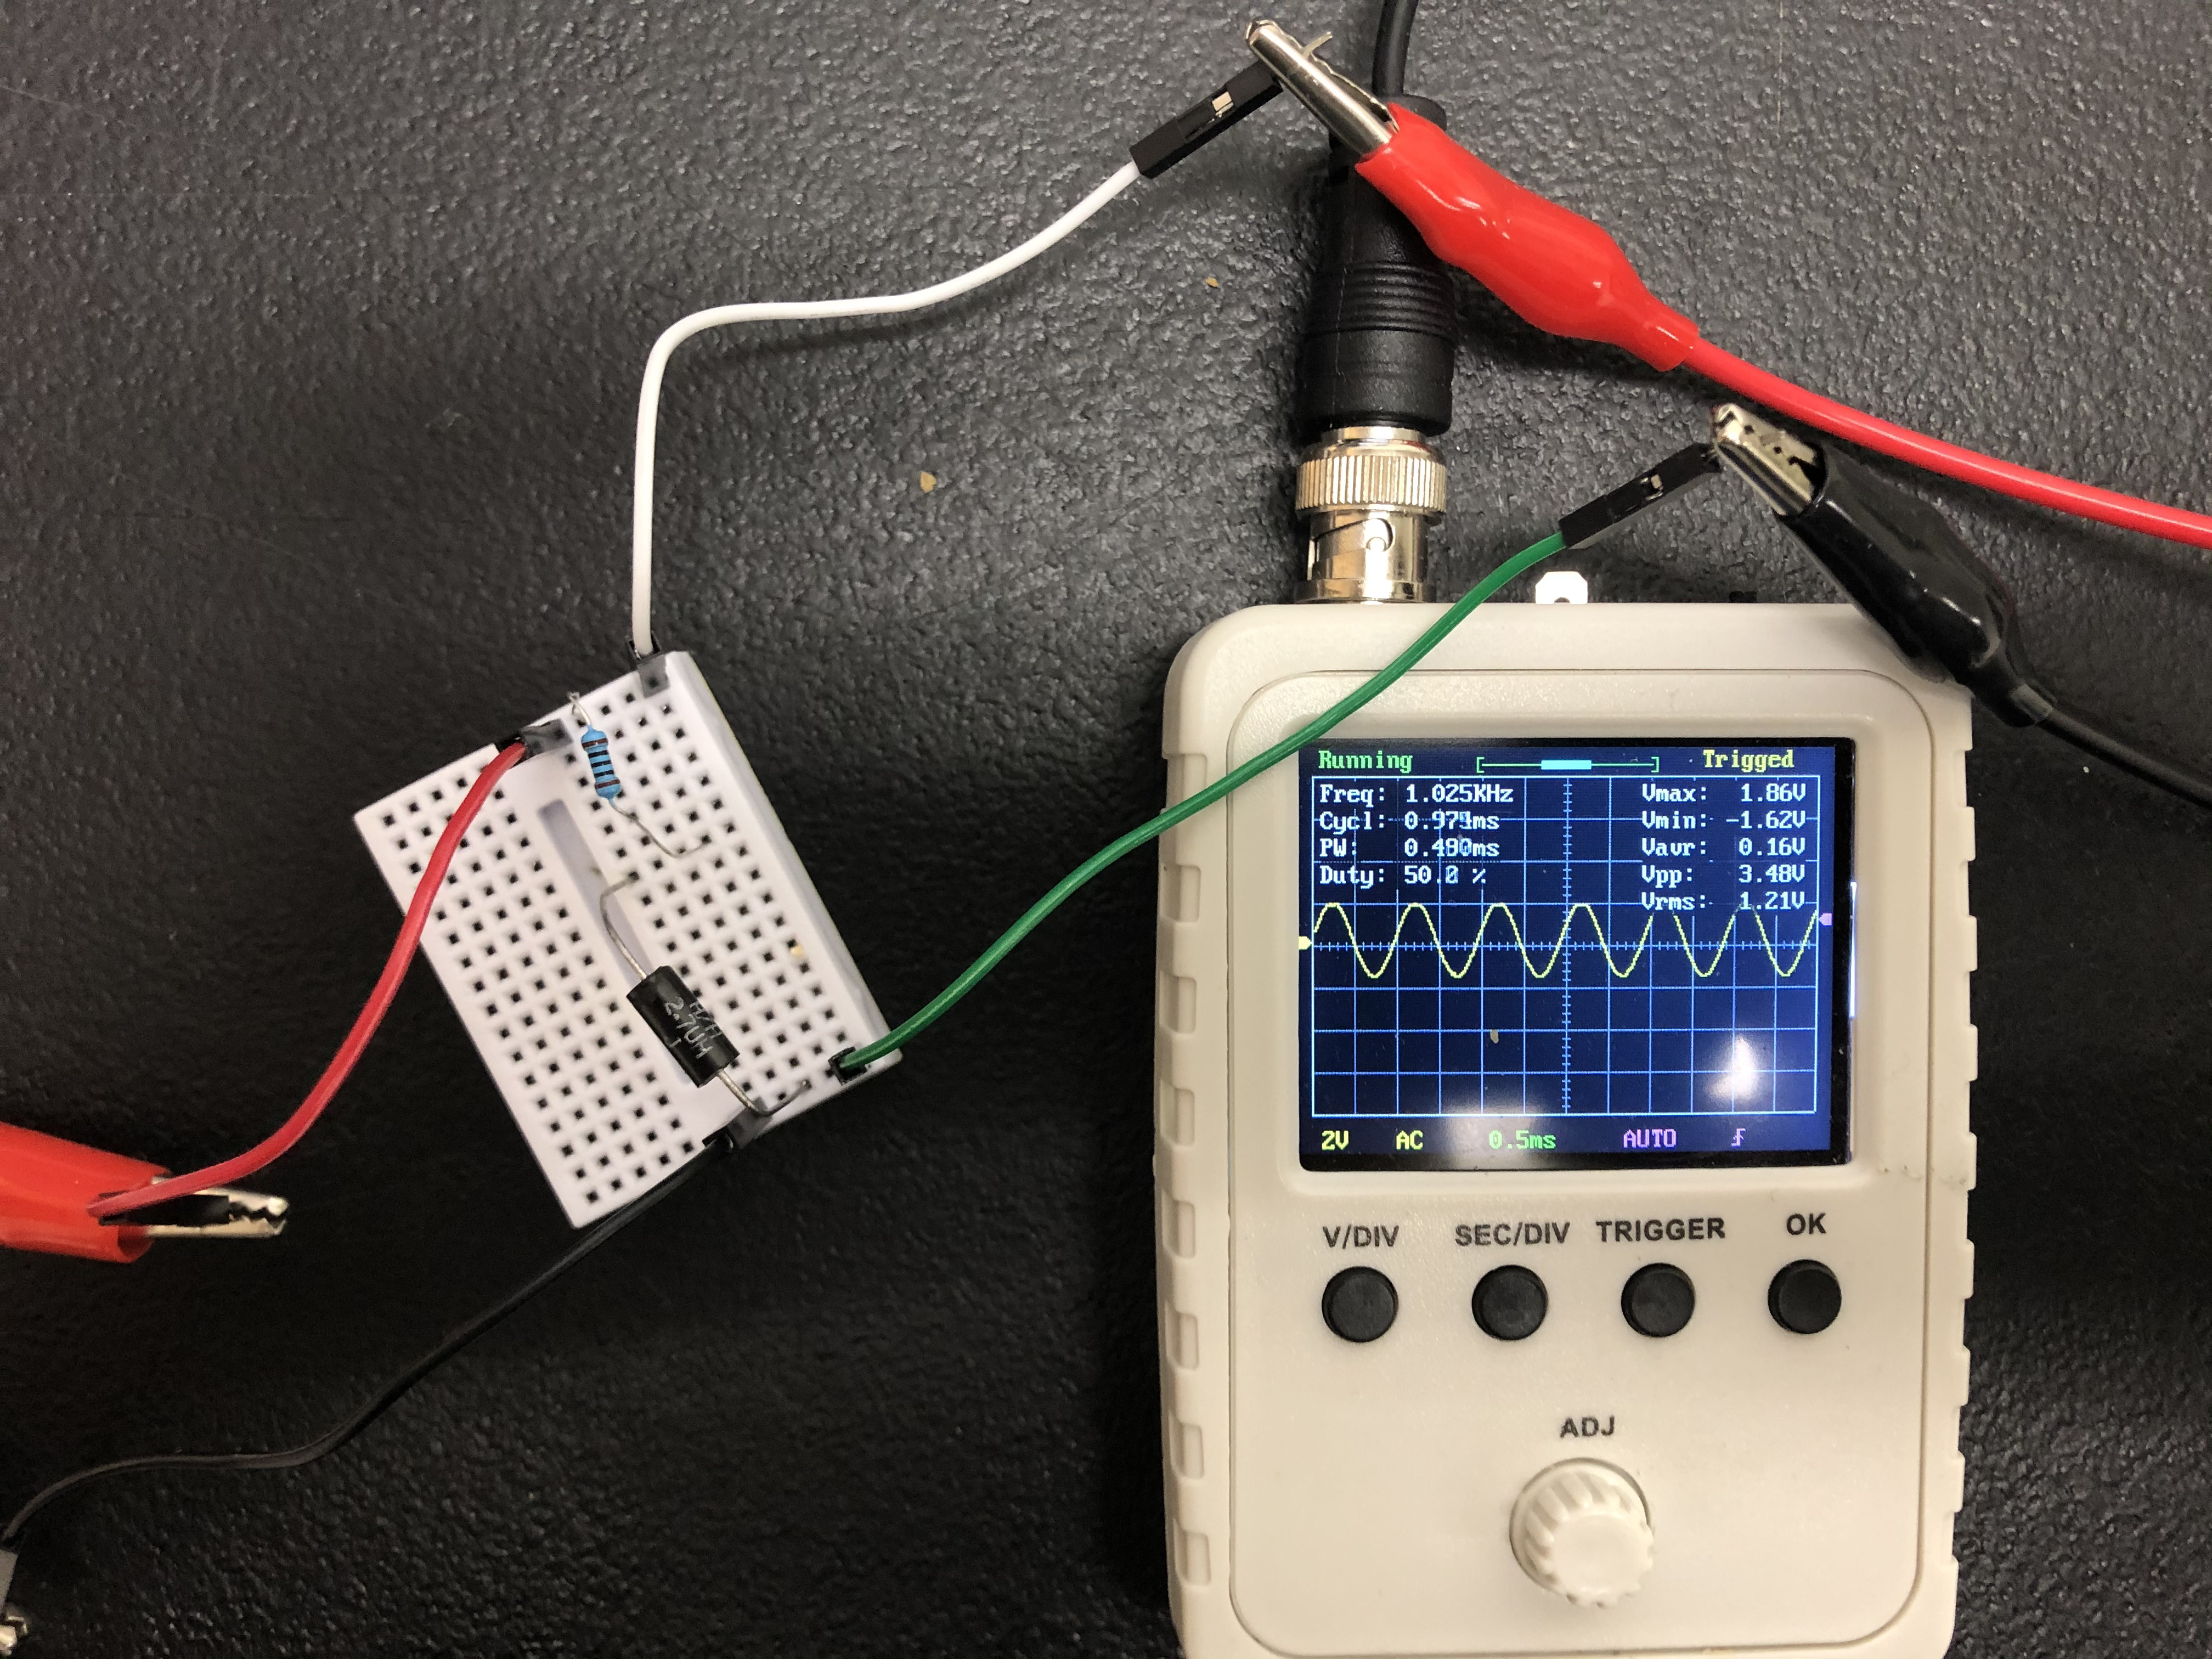
\includegraphics[scale=0.066]{V_RL.jpeg}
    \caption*{\F{V_{RL}}}\label{fig:subim1}
    \end{subfigure}
    \begin{subfigure}{0.5\textwidth}
    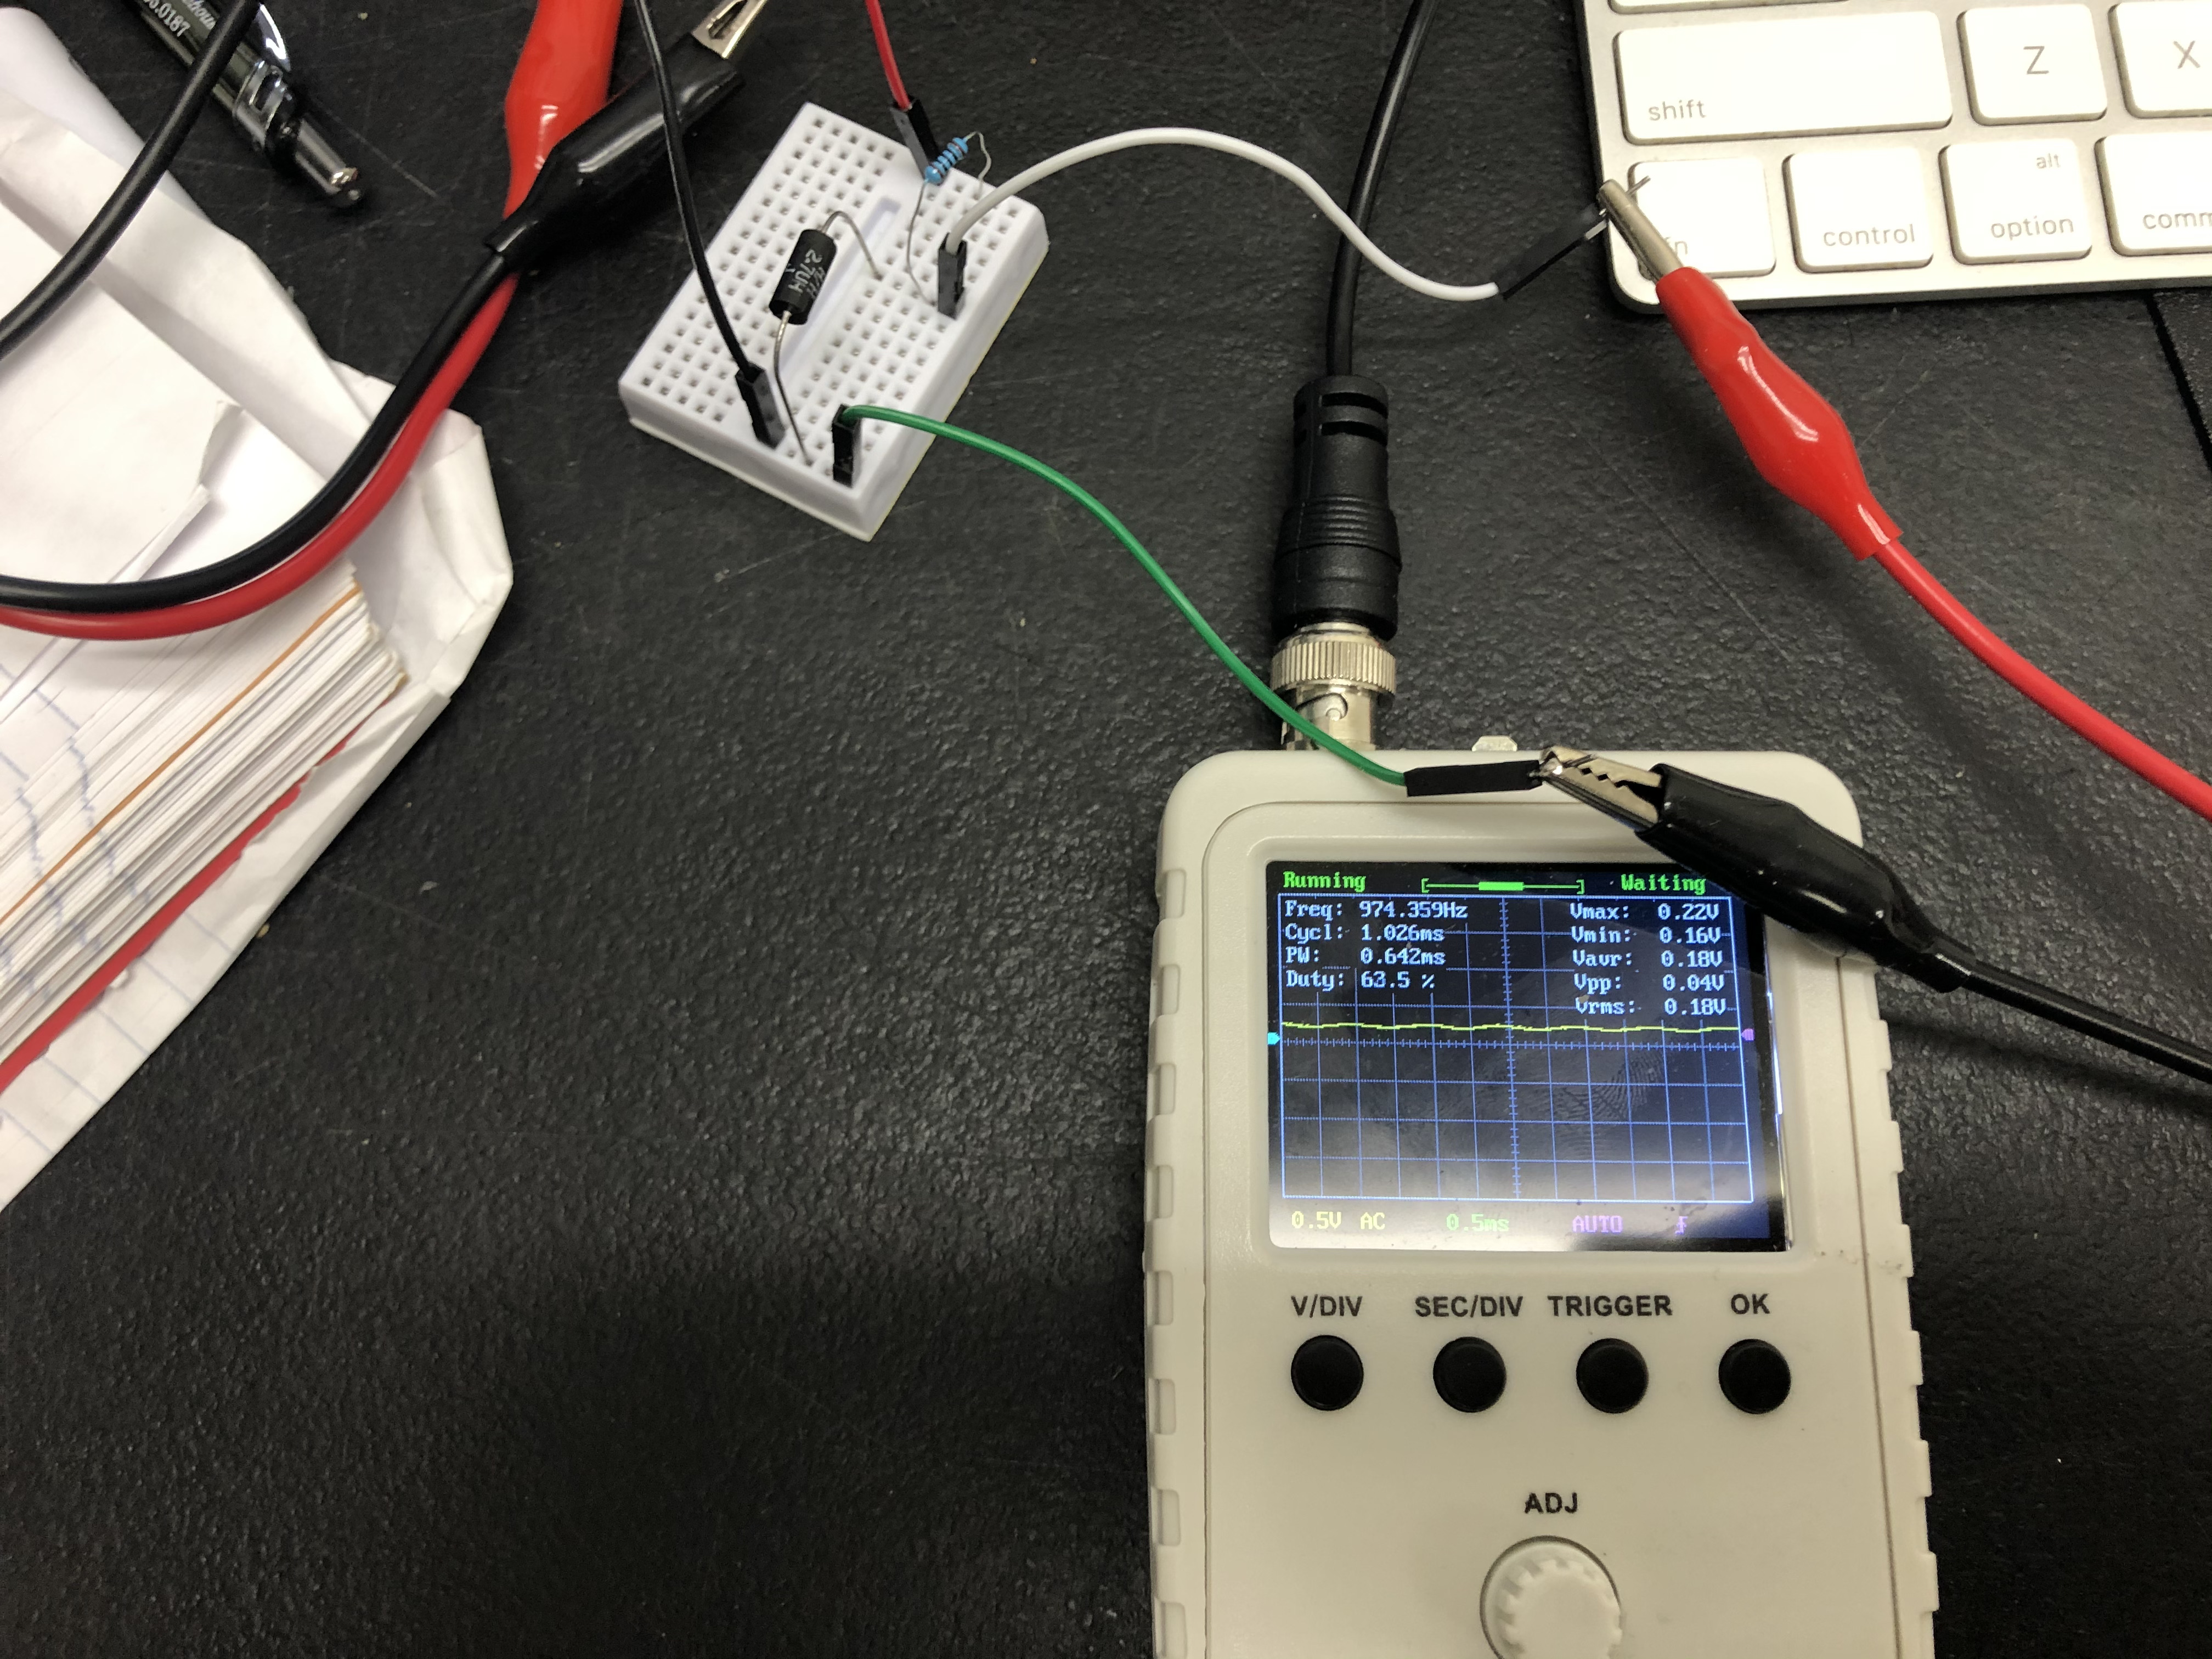
\includegraphics[scale=0.066]{V_L.jpeg}
    \caption*{\F{V_{L}}}\label{fig:subim2}
    \end{subfigure}
  \end{figure}
  \subsection*{GRAPH}
  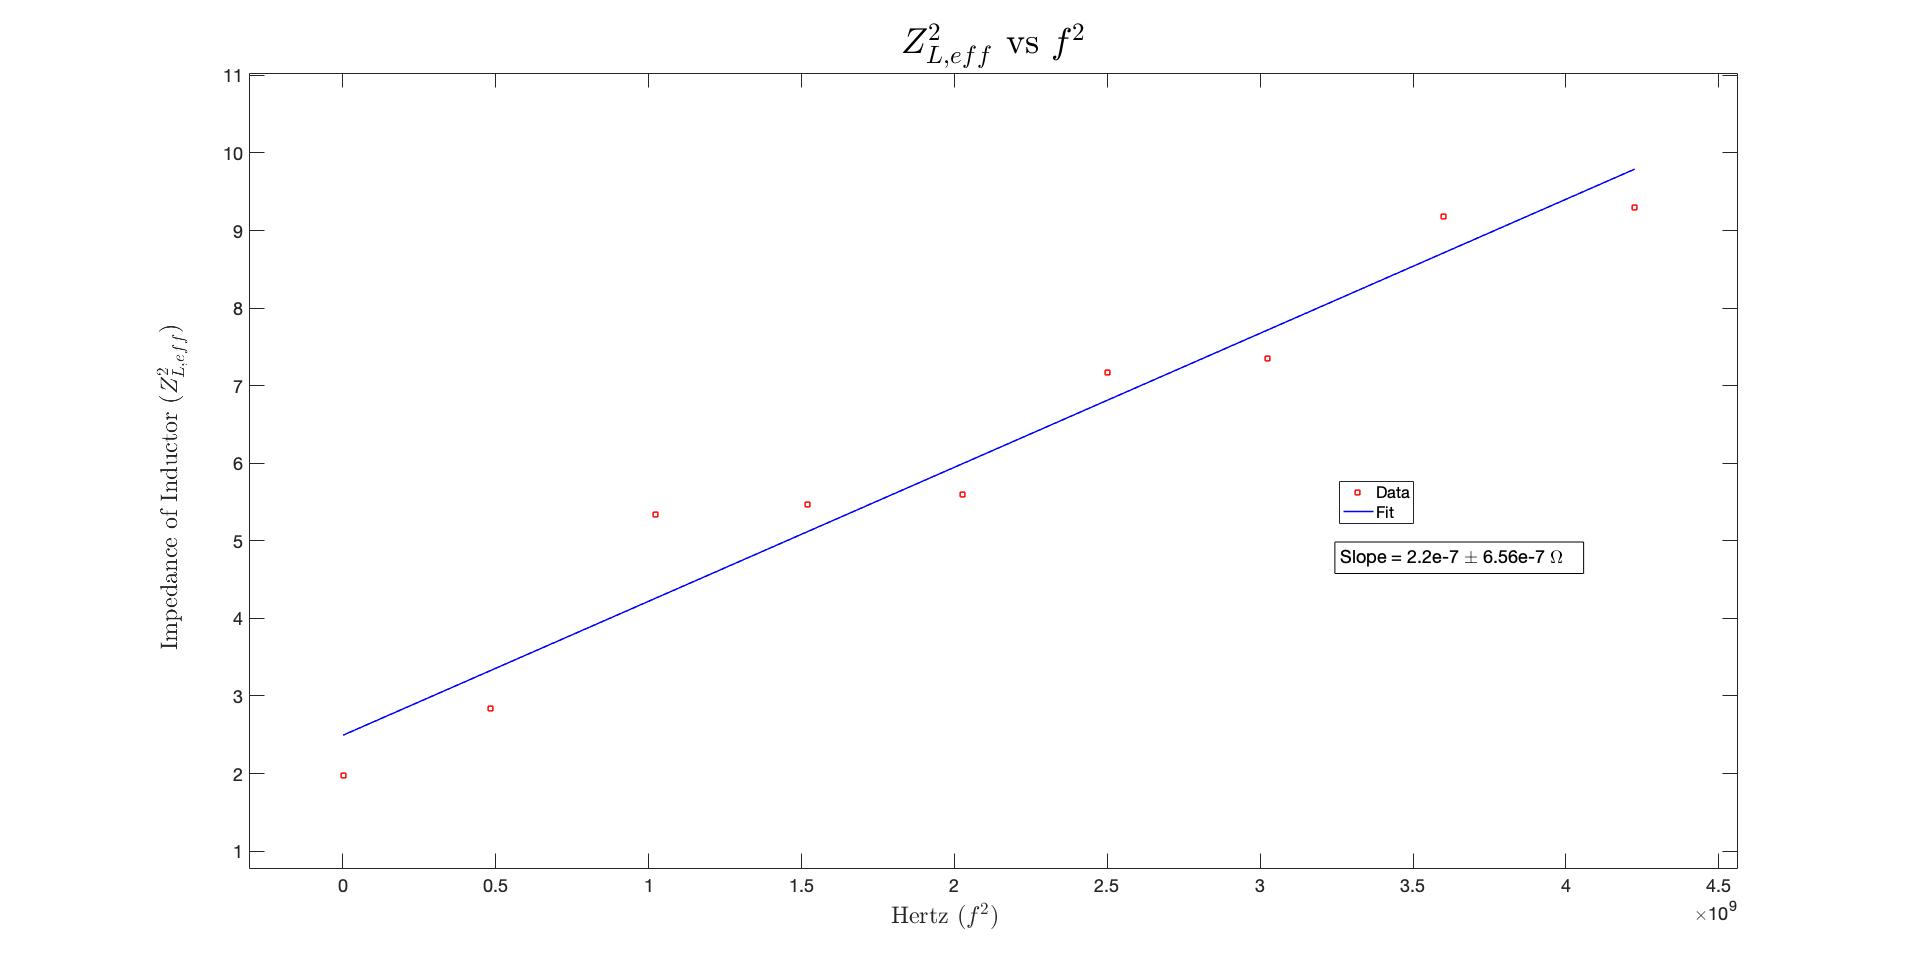
\includegraphics[width=\textwidth]{graph.jpg}
\end{center}
\begin{align*}
  R_{int} &= R/((V_{RL}/V_{L}) - 1)\\
  I_R &= V_{RL} / R\\
  Z_L &= V_L / I_R\\
  X_L &= \sqrt{ Z_L^2 - R_{int}^2}\\
  L &= X_L / (2 * pi * Hz)\\
  R &= 100\\
  Hz &= 1000,22000,32000,39000,45000,50000,55000,60000,65000\\
  R_{int} &= 1.43,1.71,2.37,2.40,2.42,2.75,2.79,3.13,3.14\\
  L &= 3.79\times{10}^{ - 5},2.27\times{10}^{ - 6},2.52\times{10}^{ - 6},2.10\times{10}^{ - 6},1.85\times{10}^{ - 6},2.01\times{10}^{ - 6},1.86\times{10}^{ - 6},2.03\times{10}^{ - 6},1.89\times{10}^{ - 6}\\
\end{align*}
\begin{itemize}
  \item We assume that the current is determined by the largest resistor in the circuit, R. How large is the error that we can expect as a result? \F{\pm\ 6.56\times{10}^{-7}\Omega}
\end{itemize}
\end{document}
